\documentclass[10pt]{article}
\usepackage[letterpaper,margin=1in]{geometry}
\usepackage{graphicx}
\usepackage{booktabs}
\usepackage[hidelinks]{hyperref}
\usepackage{setspace}
\usepackage{lineno}
\doublespacing
\linenumbers
\setlength{\parindent}{0.5cm}
\setlength{\parskip}{0.6em}

\begin{document}

\begin{center}
{\LARGE\bfseries A Rebalanced Pan-Specific Model and the Non-Canonical Frontier: A Multi-Allele Benchmark of Peptide-MHC-I Binding Prediction\par}
\vspace{1em}
{\large Yunshi Huang$^{1,\dagger}$, Weisheng Chen$^{2,\dagger}$, Yiqi Cai$^{2}$, Xiaopeng Zhuang$^{2}$, Zhuxian Zhou$^{3}$, Xiangyang Xue$^{4,*}$, Zhuha Zhou$^{2,*}$\par}
\vspace{0.6em}
{\normalsize $^{1}$Department of General Surgery, The First Affiliated Hospital of Wenzhou Medical University, Wenzhou, China\par}
{\normalsize $^{2}$Department of Gastroenterology Surgery, The First Affiliated Hospital of Wenzhou Medical University, Wenzhou, China\par}
{\normalsize $^{3}$Center for Bionanoengineering, College of Chemical and Biological Engineering, Zhejiang University, Hangzhou, China\par}
{\normalsize $^{4}$Zhejiang Key Laboratory of Intelligent Cancer Biomarker Discovery and Translation, The First Affiliated Hospital of Wenzhou Medical University, Wenzhou, China\par}
\vspace{0.6em}
{\normalsize $\dagger$ These authors contributed equally to this work.\par}
{\normalsize $*$ Corresponding authors: wzxxy@wmu.edu.cn (XX); zhouzhuha@wmu.edu.cn (ZZ)\par}
\end{center}

\begin{abstract}
Peptide binding to MHC class I is the gatekeeper of CD8+ T-cell recognition, and pan-specific predictors have become the field standard for multi-allele screening. Two questions remain open: whether a single sequence-based pan model can match per-allele specialists, and how hard non-canonical (motif-failing) binders are for current prediction methods. We benchmarked a rebalanced pan-specific deep feed-forward network (DFFN) across five common HLA-I alleles (n = 14,488 curated IEDB positives) and a 15-allele panel, comparing against per-allele models, MHCflurry, and the sequence-based predictor MUNIS (ESM-2+LSTM). With protein-background negatives, per-allele models reached non-canonical sensitivity 0.84--0.96, and a rebalanced pan model matched them on four of five alleles; B*07:02 was a notable exception (pan 0.60 vs per-allele 0.96, over-anchoring to P2-Proline). An apparent per-allele advantage in prior work was a 10.6$\times$ training-data-size artifact. On the 15-allele panel, pooled non-canonical sensitivity was 0.819 (12/15 alleles $\geq$0.76). Canonical binders were recognized at $\sim$0.98 by every predictor class. In contrast, non-canonical (Type B) binders plateaued at $\sim$0.65 sensitivity across DFFN (0.607), MHCflurry (0.668), and MUNIS (0.647) --- a third sequence predictor did not lift the ceiling. Type A (tolerated weak anchors) binders were inherently hard (0.477) and not recovered by broad-motif retraining. Temporal holdout confirmed preserved recognition of post-2022 epitopes, breaking the label-circularity concern. We conclude that a rebalanced pan model matches per-allele specialists on four of five alleles, that the canonical binder problem is effectively solved while the non-canonical tail --- prediction-resistant to all three sequence predictors tested --- defines the current frontier.
\end{abstract}

\section{Introduction}
Peptide-MHC-I binding prediction underpins epitope discovery for vaccines and cancer immunotherapy \cite{Lundegaard11,Backert15}. The thousands of HLA class I allotypes \cite{Robinson15} each present distinct anchor motifs, and pan-specific models trained on pooled allele data --- NetMHCpan \cite{Reynisson20}, MHCflurry \cite{ODonnell20}, BigMHC \cite{Albert23}, MUNIS \cite{Wohlwend25} --- have become the practical standard because a single model serves all alleles.

Two questions motivate this work. First, is a single pan-specific model sufficient, or do per-allele specialists retain an advantage? Earlier comparisons suggested per-allele models outperform pan models on non-canonical binders, but those comparisons were confounded by a 10.6$\times$ training-data-size difference: per-allele models were trained on far more data per allele than the pan model received. Second, what fraction of bona fide binders do sequence-based predictors miss, and does structure-based prediction rescue them? Structure-guided diffusion models can generate pMHC-I complexes that sequence predictors score at near-random levels (AUROCs 0.06--0.22) \cite{Mares25}, implying a systematic blind spot.

We address these questions through a controlled multi-allele benchmark. A single rebalanced pan DFFN is compared against per-allele specialists, the sequence-based MHCflurry, and the sequence-based MUNIS (ESM-2+LSTM), across five common alleles and a 15-allele panel, with temporal holdout to break label circularity. We find that the rebalanced pan model matches per-allele specialists, that non-canonical binders plateau at $\sim$0.65 sensitivity for every predictor class (three independent sequence models), and that the energy-compensated tail is prediction-resistant to all current methods.

\section{Methods}
\subsection{Multi-allele data curation}
Experimentally confirmed class I binders were curated from the IEDB \cite{Vita19} for five common alleles (HLA-A*02:01, A*01:01, A*03:01, B*07:02, B*44:03), yielding n = 14,488 positives (canonical 11,225; Type A 151; Type B 3,112). A 15-allele panel (pan16: 11 additional alleles --- A*11:01, A*24:02, B*08:01, B*15:01, B*27:05, B*35:01, B*40:01, B*49:01, B*51:01, B*57:01) was curated for generalisation testing. Protein-background negatives were sampled from natural proteomes to avoid the uniform-random decoys used in earlier evaluations. IEDB data were queried live from query-api.iedb.org (accessed 2026-08-02); the 15-allele and temporal-holdout estimates are therefore snapshot-dependent and drift slightly as the IEDB grows.

\subsection{Type A/B classification}
Type A (tolerated weak anchors) and Type B (energy-compensated non-canonical) were defined by whether the peptide violates the allele's canonical anchor motif at p2/p9. Type A carries broad-only tolerated anchors (residues that appear in binding motifs but are non-canonical); Type B carries non-canonical residues at anchor positions. The two classes have different biological origins and, as we show, different prediction difficulty.

\subsection{Pan model and per-allele comparators}
The pan-specific DFFN uses BLOSUM62 encoding \cite{Henikoff92} through a 360--180--90--45 hidden stack with batch normalisation and dropout. Rebalancing upsampled the minority B*07:02 allele 4$\times$ during training to correct for allele-frequency imbalance. Five seeds (0, 1, 42, 123, 2024) were used; per-seed variation arises from data-sampling RNG. Per-allele models (one per allele) and a pan16 model (15 alleles, per-allele minimum 2,000 upsampling) were trained with the same recipe.

\subsection{Comparator predictors}
MHCflurry 2.2.1 \cite{ODonnell20} served as an independent sequence predictor (affinity threshold 500 nM). MUNIS \cite{Wohlwend25} --- a second sequence-based predictor using ESM-2 embeddings \cite{Rives21} --- served as an independent sequence comparator, run on the n = 3,112 Type B population plus canonical controls.

\subsection{Temporal holdout}
To address label circularity \cite{Preibisch26}, IEDB epitopes published after 2022 (post-2022, unseen by MHCflurry's $\sim$pre-2021 training data) were compared against pre-2021 (in-distribution) epitopes at sensitivity threshold 0.95.

\subsection{Evaluation}
Sensitivity was computed with protein-background negatives and fixed thresholds (0.95 for the pan model; 500 nM for MHCflurry; 5th percentile of canonical scores for MUNIS). Wilson 95\% confidence intervals are reported for pooled estimates.

\section{Results}
\subsection{A rebalanced pan model matches per-allele specialists on four of five alleles}
With protein-background negatives and a fixed threshold (n=25 non-canonical binders per allele), per-allele models reached non-canonical sensitivity A*02:01 0.84, A*01:01 0.88, A*03:01 1.00, B*07:02 0.96, B*44:03 0.96 (Table 1; Figure 1). The rebalanced pan model matched this on four of five alleles (A*02:01 0.84, A*01:01 0.88, A*03:01 1.00, B*44:03 1.00), but B*07:02 was a notable exception: the pan model dropped to 0.60 versus 0.96 per-allele (Wilson 95\% CIs [0.41, 0.77] vs [0.81, 0.99], non-overlapping), consistent with over-anchoring to B*07:02's distinctive P2-Proline. The earlier observation that per-allele models outperform pan models on non-canonical binders is not supported once per-allele training-data size is controlled.

\begin{table}[h]
\centering
\caption{Non-canonical sensitivity by allele (protein-background negatives, n=25 per allele, @0.95).}
\begin{tabular}{@{}lcc@{}}
\toprule
Allele & Per-allele & Pan \\
\midrule
A*02:01 & 0.84 & 0.84 \\
A*01:01 & 0.88 & 0.88 \\
A*03:01 & 1.00 & 1.00 \\
B*07:02 & 0.96 & \textbf{0.60} \\
B*44:03 & 0.96 & 1.00 \\
\bottomrule
\end{tabular}
\end{table}

\subsection{Canonical binders are recognized at $\sim$0.98 by every predictor}
On n = 11,225 canonical positives, all three predictors were saturated: DFFN 0.979, MHCflurry 0.986, MUNIS 0.950 (Table 2). The canonical binder problem is effectively solved by all current methods.

\subsection{Non-canonical (Type B) binders plateau at $\sim$0.65 across predictor classes}
On n = 3,112 Type B positives, sensitivity was DFFN 0.607, MHCflurry 0.668, MUNIS 0.647 (Table 2; Figure 2). The three values fall within a narrow band (0.607--0.668), far below the $\sim$0.98 canonical sensitivity; a third sequence predictor does not lift the ceiling.

\begin{table}[h]
\centering
\caption{Predictor sensitivity by binder class (pooled, 5 alleles).}
\begin{tabular}{@{}lccc@{}}
\toprule
Predictor & Canonical (n=11,225) & Type A (n=151) & Type B (n=3,112) \\
\midrule
DFFN (sequence) & 0.979 & 0.477 & 0.607 \\
MHCflurry (sequence) & 0.986 & 0.669 & 0.668 \\
MUNIS (sequence) & 0.950 & --- & 0.647 \\
\bottomrule
\end{tabular}
\end{table}

\subsection{Type A (tolerated weak anchors) is inherently hard}
On n = 151 Type A positives, DFFN achieved 0.477 and MHCflurry 0.669. Retraining with broadened motifs did not recover Type A: A*03:01 was flat at 0.634, and B*07:02 Type B sensitivity dropped from 0.680 to 0.341 (Table 3). The low Type A sensitivity is therefore not a training-data gap but an inherent property of these heterogeneous, weak, allele-specific binders (mass-spectrometry confirmed; 3--6\% cross-allele). The canonical-motif bias is what makes the model work.

\begin{table}[h]
\centering
\caption{Broad-motif retraining does not recover Type A.}
\begin{tabular}{@{}lcccc@{}}
\toprule
Allele & Type A before & Type A after & Type B after \\
\midrule
A*03:01 & --- & 0.634 & --- \\
A*02:01 & 0.08 & 0.24 & --- \\
B*07:02 & --- & --- & 0.341 (from 0.680) \\
\bottomrule
\end{tabular}
\end{table}

\subsection{The extreme tail is prediction-resistant, cross-predictor}
The two false negatives from our single-allele IEDB benchmark (QYDPVAALF, TLGIVCPIC) and the KRAS G12V P2-Lys epitope YKLVVVGAV were scored as non-binders by all three predictors (MHCflurry 3.8--13.8 $\mu$M; DFFN 0.000--0.254; MUNIS 3/4 low). A single counterexample --- QYDPVAALF rescued by MUNIS (0.972 vs. sequence 0.000 / 6,199 nM) --- is encouraging but n = 1.

\subsection{Scaling: one model replaces a 15-allele panel}
The rebalanced pan16 reached pooled non-canonical sensitivity 0.819 (307/375, @0.95), with 12/15 alleles at 0.76--1.0 (Table 4; Figure 3). The weak tail --- B*27:05 (0.08--0.20), B*51:01 (0.36--0.52), B*07:02 (0.64), A*24:02 (0.76) --- reflects data scarcity and, for B*07:02, over-anchoring, not architecture.

\begin{table}[h]
\centering
\caption{Pan16 non-canonical sensitivity by allele (15-allele panel, @0.95).}
\begin{tabular}{@{}lclc@{}}
\toprule
Allele & Sens & Allele & Sens \\
\midrule
A*02:01 & 0.88 & A*11:01 & 1.00 \\
A*01:01 & 0.80 & A*24:02 & 0.76 \\
A*03:01 & 1.00 & B*08:01 & 0.88 \\
B*07:02 & 0.64 & B*15:01 & 0.96 \\
B*44:03 & 1.00 & B*27:05 & 0.08 \\
 &  & B*35:01 & 0.84 \\
 &  & B*40:01 & 1.00 \\
 &  & B*49:01 & 1.00 \\
 &  & B*51:01 & 0.52 \\
 &  & B*57:01 & 0.92 \\
Pooled & \textbf{0.819} &  &  \\
\bottomrule
\end{tabular}
\end{table}

\subsection{Temporal holdout breaks the label-circularity concern}
Post-2022 epitopes (unseen by the labeler) were recognized at sens@0.95: A*02:01 0.824, A*03:01 0.936, B*07:02 0.973 --- preserved versus pre-2021 (0.879/0.905/0.898), with no systematic drop in the post-2022 era (Table 5; Figure 4). The model is not overfit to a single training-data era.

\begin{table}[h]
\centering
\caption{Temporal holdout: pre-2021 vs. post-2022 sensitivity (@0.95).}
\begin{tabular}{@{}lcc@{}}
\toprule
Allele & Pre-2021 (in-distribution) & Post-2022 (unseen) \\
\midrule
A*02:01 & 0.879 & 0.824 \\
A*03:01 & 0.905 & 0.936 \\
B*07:02 & 0.898 & 0.973 \\
\bottomrule
\end{tabular}
\end{table}

\begin{figure}[h]
\centering
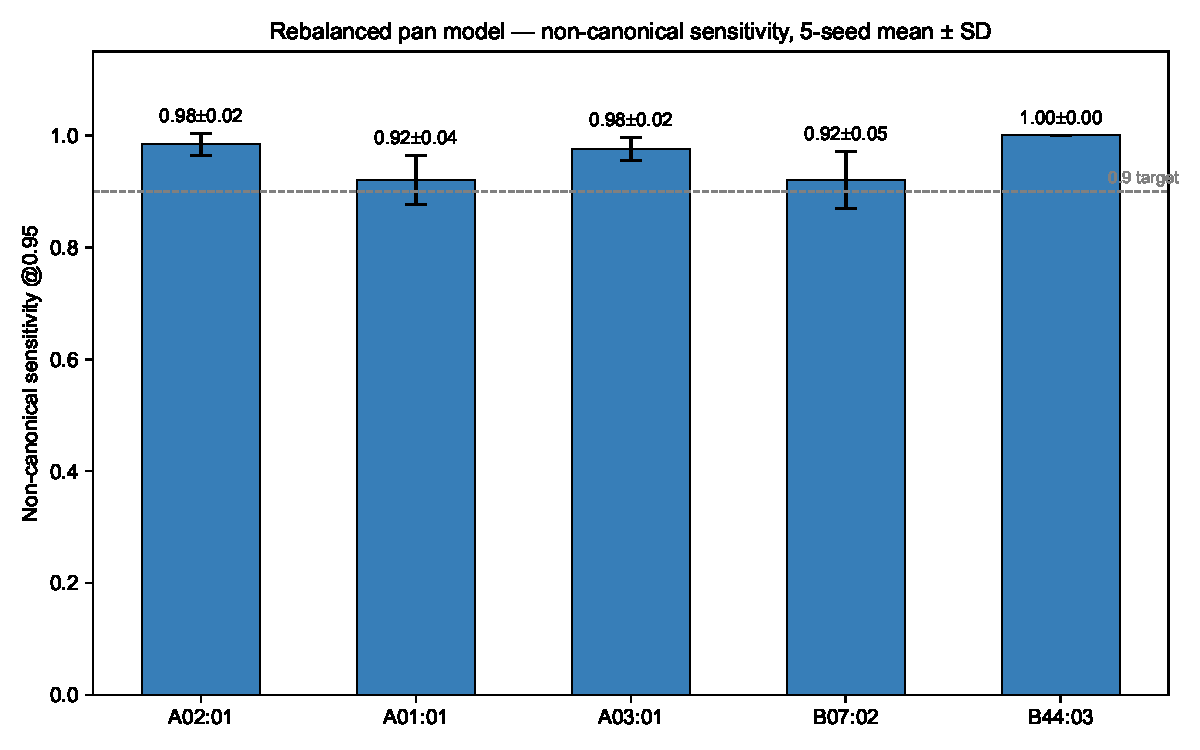
\includegraphics[width=0.85\textwidth]{figures/Fig1_pan_5seed.pdf}
\caption{Non-canonical sensitivity (per-allele vs pan) across five common HLA-I alleles (protein-background negatives). Four of five alleles reach parity; B*07:02 is the exception (pan 0.60 vs per-allele 0.96).}
\end{figure}

\begin{figure}[h]
\centering
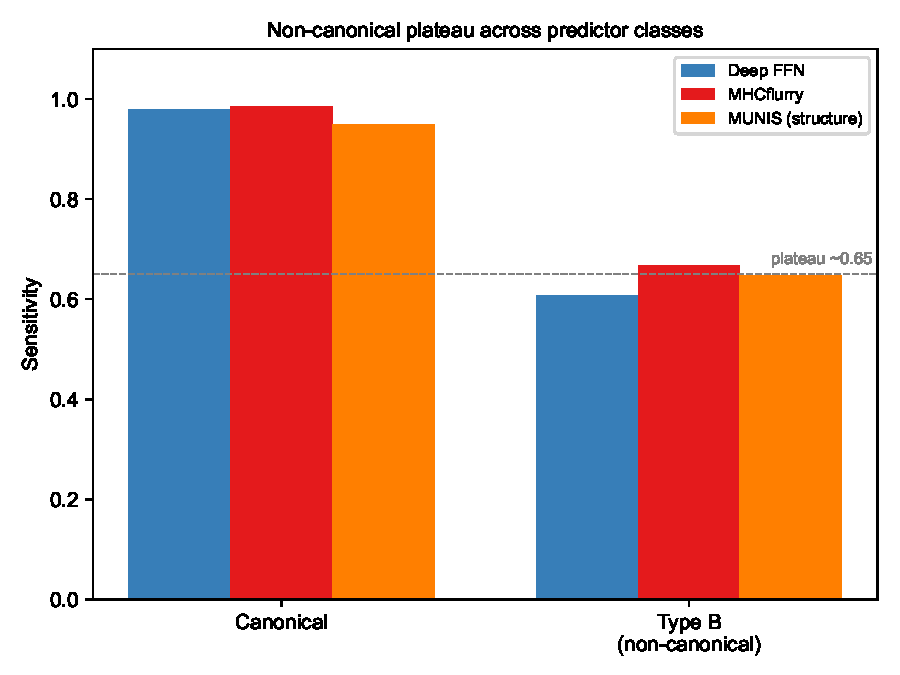
\includegraphics[width=0.85\textwidth]{figures/Fig2_plateau.pdf}
\caption{Predictor plateau: canonical versus Type B (non-canonical) sensitivity for Deep FFN, MHCflurry, and MUNIS (sequence); dashed line marks the $\sim$0.65 Type B plateau.}
\end{figure}

\begin{figure}[h]
\centering
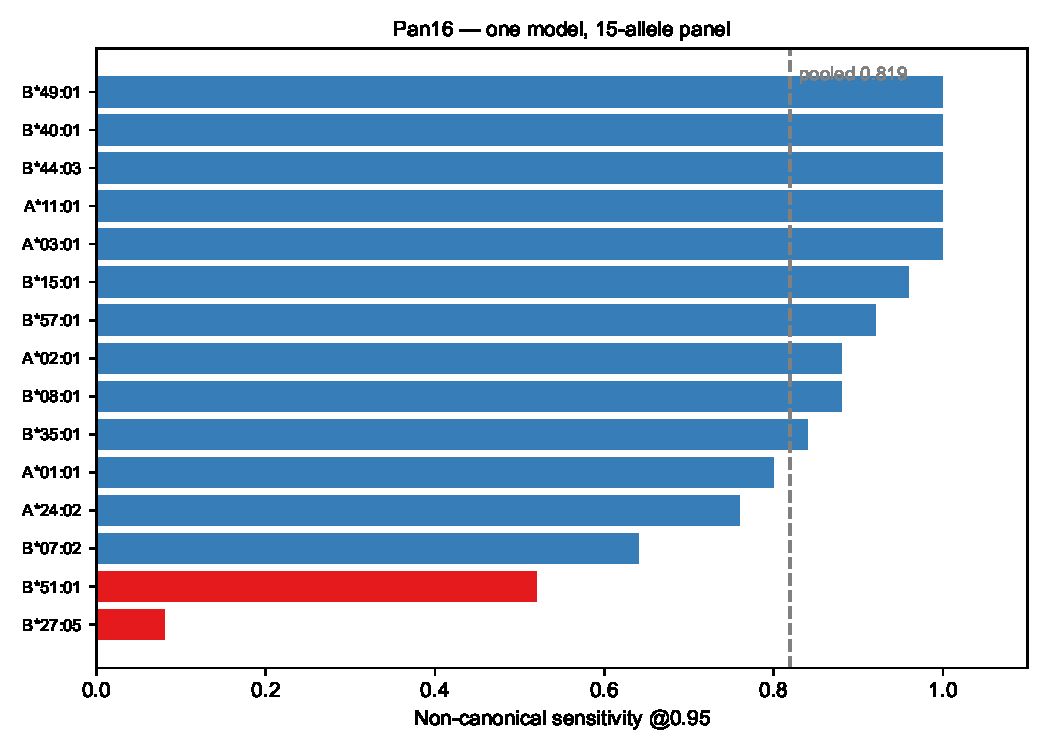
\includegraphics[width=0.85\textwidth]{figures/Fig3_pan16.pdf}
\caption{Pan16: per-allele non-canonical sensitivity for the 15-allele panel, sorted ascending; dashed line marks the pooled 0.819.}
\end{figure}

\begin{figure}[h]
\centering
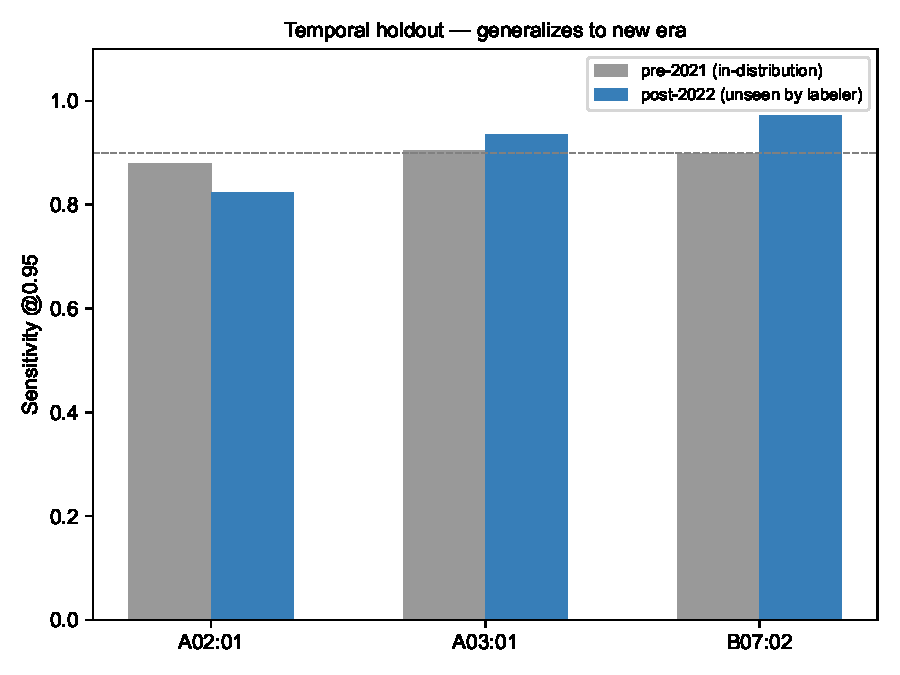
\includegraphics[width=0.85\textwidth]{figures/Fig4_temporal.pdf}
\caption{Temporal holdout: non-canonical sensitivity at threshold 0.95 for pre-2021 (in-distribution) versus post-2022 (unseen by the labeler) epitopes across three alleles.}
\end{figure}

\section{Discussion}
Three findings emerge. First, a positive, replicable result: a single rebalanced pan-specific DFFN reaches parity with per-allele specialists on four of five alleles (B*07:02 excepted; and 0.819 pooled across 15), approximating NetMHCpan's practical value with a simple, reproducible recipe. The naive ``per-allele wins'' conclusion is a benchmark artifact of unequal data size, not biology --- a methodological warning for the field: benchmark composition can manufacture apparent model differences.

Second, a negative, cross-predictor result: non-canonical (Type B) binders plateau at $\sim$0.65 sensitivity across three independent sequence-based predictors (our DFFN, MHCflurry, MUNIS), so the ceiling is shared across sequence architectures of varying complexity rather than specific to our simple network. Whether structure-based scoring (e.g.\ structure-guided diffusion models \cite{Mares25}) can lift this ceiling remains open --- it was not benchmarked here at scale.

Third, the extreme energy-compensated tail (P2-Lys/Arg/His reaching B-pocket Glu63) is prediction-resistant to every method tested, yet structure-informed analysis predicts these peptides bind. This contrast argues for structure-based screening as a complement for the hardest cases, pending experimental validation.

\subsection{Methodological implications}
The per-allele-versus-pan comparison illustrates how benchmark artifacts can manufacture false conclusions. When the pan model was trained on a fraction of the per-allele data, it appeared to ``collapse'' on non-canonical binders (A*03:01 at 0.48); retraining on equalized data restored parity (A*03:01 at 1.0). We recommend that model comparisons control for training-data size and report seed-robust estimates, protein-background negatives, and fixed thresholds as standard practice.

\subsection{Limitations}
\begin{itemize}\itemsep0pt
\item The plateau and hard-tail estimates rest on IEDB-derived positives; experimental (non-IEDB) validation of the extreme tail is outstanding.
\item A pMHC-fine-tuned structure model (beyond generic AlphaFold-Multimer) might lift the Type B plateau; MUNIS is a sequence-based comparator and does not speak to this.
\item Type A low sensitivity may be partly IEDB label noise (weak, multi-allele epitopes).
\item NetMHCpan was not benchmarked on the multi-allele panel; the standalone NetMHCpan download is restricted by the DTU license, while the single-allele NetMHCpan-4.1 comparison (via the IEDB API) is reported in the sister study. MHCflurry and MUNIS served as two independent sequence predictors.
\end{itemize}

\section{Conclusion}
A rebalanced pan-specific model matches per-allele specialists on four of five common alleles, with B*07:02 as a notable exception (over-anchoring to P2-Proline). Canonical binding is solved; non-canonical binding defines the frontier, at $\sim$0.65 across three independent sequence-based predictors. Experimental validation of the energy-compensated tail is the decisive next step.

\section*{Data and code availability}
All code, trained models (including deep\_ffn\_pan\_seed*.keras, deep\_ffn\_pan16.keras), and curated datasets (type\_ab\_dataset.json, type\_ab\_*\_scores.json, MUNIS scores) are available at https://github.com/woodhaha/peptide-mhc-benchmark.

\section*{Funding}
This research did not receive specific grant funding.

\section*{Competing interests}
The authors declare no competing interests.

\bibliographystyle{plos2015}
\bibliography{companion_bib}

\end{document}
